%------------------------------------------------------------------------------------
% CouseTeX Simplified Latex Lightweight Open Course Web-framework
% [shane.transue@ucdenver.edu]
%------------------------------------------------------------------------------------
\documentclass[10pt]{article}
%------------------------------------------------------------------------------------
% CouseTeX Simplified Latex Lightweight Open Course Web-framework
% [shane.transue@ucdenver.edu]
%------------------------------------------------------------------------------------
\usepackage[top=0.7in, bottom=1.0in, left=0.8in, right=1.0in]{geometry}
\usepackage{changepage}
\usepackage{listings}
\usepackage{color}
\usepackage[T1]{fontenc}
\usepackage{hyperref}

%------------------------------------------------------------------------------------
% CouseTeX Simplified Latex Lightweight Open Course Web-framework
% [shane.transue@ucdenver.edu]
%------------------------------------------------------------------------------------
\lstdefinestyle{customc}{
    basicstyle=\ttfamily,
    language=C,
	rulecolor=\color{red}, 
    keywordstyle=\rmfamily\bfseries,
    commentstyle=\itshape\color{green},
	stringstyle=\color{green}
}
\lstset{style=customc}

\newenvironment{codelisting}
{\HCode{<div class="codelisting" style="padding: 2px;">}}
{\HCode{</div>}}

%------------------------------------------------------------------------------------
% CouseTeX Simplified Latex Lightweight Open Course Web-framework
% [shane.transue@ucdenver.edu]
%------------------------------------------------------------------------------------

%------------------------------------------------------------------------------------
% This complex set of macros redefines a div hierarchy within the generated
% html so that section headers and section content can have two different
% CSS styles.
%------------------------------------------------------------------------------------
\let\oldsection\section
\newenvironment{testSection}
{\HCode{<div class="section">} \oldsection}
{\HCode{</div>}}

\renewenvironment{section}[1]
{\testSection{#1} \HCode{<div class="sectionContent">}}
{\HCode{</div></div>}}

\let\oldsubsection\subsection
\newenvironment{testSubSection}
{\HCode{<div class="section">} \oldsubsection}
{\HCode{</div>}}

\renewenvironment{subsection}[1]
{\testSubSection{#1} \HCode{<div class="sectionContent">}}
{\HCode{</div></div>}}



\usepackage{graphicx}
\usepackage{amsmath}

\begin{document}
%------------------------------------------------------------------------------------
% CouseTeX Simplified Latex Lightweight Open Course Web-framework
% [shane.transue@ucdenver.edu]
%------------------------------------------------------------------------------------
%------------------------------------------------------------------------------------
% CouseTeX Simplified Latex Lightweight Open Course Web-framework
% [shane.transue@ucdenver.edu]
%------------------------------------------------------------------------------------

%------------------------------------------------------------------------------------
% Page Style
%------------------------------------------------------------------------------------
\Css{body {
	background-color: \#fff;
	margin: 0 0 0 0;
	}
}

\Css{body > p.noindent{
	height 0px;
	margin: 0 0 0 0;
}}

\Css{div.topbar {
	margin: 0 0 0 0;
	margin-bottom: 8px;
	background-color: \#5e5e5e;
	height: 6px;
	}
}

\Css{img.math {
	vertical-align: top;
	margin-top: -6px;
	}
}

\Css{table.equation {
	padding-top: 10px;
	}
}

%------------------------------------------------------------------------------------
% Links
%------------------------------------------------------------------------------------
\Css{a:link {
	color: \#a0a0a0;
	text-decoration: none;
	}
}

\Css{a:hover {
	color: black;
	text-decoration: none;
	}
}

\Css{a:visited:hover {
	color: black;
	text-decoration: none;
	}
}

\Css{a:visited {
	color: \#a0a0a0;
	text-decoration: none;
	}
}

%------------------------------------------------------------------------------------
% Syntax Highlighting
%------------------------------------------------------------------------------------
\Css{div.lstinputlisting .ectt-1000 {
	font-family: monospace; 
	color:black;
	}
}

% Comment
\Css{div.lstinputlisting .ecit-1000 {
	font-family: monospace;
	color: \#00a00b;
	}
} 

% Keyword
\Css{div.lstinputlisting .ecbx-1000 {
	font-family: monospace;
	color: \#0084ff;
	}
}

\Css{div.caption {
	color: black;
	}
}

\Css{div.codelisting {
	background: \#fafafa;
	border: 1px solid \#f0f0f0;
	font-size: 13px;
	}
}

\Css{div.lstinputlisting {
	margin: 4px;
	padding-bottom: 8px;
	border: 1px solid \#f0f0f0;
	background: \#fff;
	font-size: 13px;
	}
}

%------------------------------------------------------------------------------------
% Section Style [Shadow: http://www.cssmatic.com/box-shadow]
%------------------------------------------------------------------------------------
\Css{div.section{
	margin: 4px;
	margin-top: 8px;
	padding-top: 4px;
	padding-left: 4px;
	background: \#fafafa;
	border: 1px solid \#f0f0f0;
	font-family: "Arial", Verdana, sans-serif;
	-webkit-box-shadow: 0px 0px 9px 2px rgba(0,0,0,0.05);
	-moz-box-shadow: 0px 0px 9px 2px rgba(0,0,0,0.05);
	box-shadow: 0px 0px 9px 2px rgba(0,0,0,0.05);
	}
}

\Css{div.sectionContent {
	padding: 4px;
	font-family: "Times New Roman", Times, Serif;
	font-size: 17px;
	}
}

\Css{.sectionHead {
	margin-left: 10px;
	margin-top: -8px;
	margin-bottom: -10px;
	}
}

\Css{.subsectionHead {
	margin-left: 10px;
	margin-top: -8px;
	margin-bottom: -10px;
	}
}

\Css{.noindent {
	margin-left: 6px;
	}
}

% Figure
\Css{hr.figure {
	border: 1px solid \#ddd;
	}
}

\Css{hr.endfigure {
	border: 1px solid \#ddd;
	}
}

%------------------------------------------------------------------------------------
% CouseTeX Simplified Latex Lightweight Open Course Web-framework
% [shane.transue@ucdenver.edu]
%------------------------------------------------------------------------------------

\HCode {
	<div class="topbar">&nbsp;</div>
	<div class="title">
		<strong>CSCI-4800/5800 Shader and GPU Programming</strong>
	</div>
	<div id="colortab" class="bluetabs">
			<ul>
				<li><a href="index.html" title="Home"><span>Home</span></a></li>
				<li><a href="index.html" title="Syllabus"><span>Syllabus</span></a></li>
				<li><a href="#" title="Lectures" rel="lectures_menu"><span>Lectures</span></a></li>
				<li><a href="#" title="Modules" rel="modules_menu"><span>Modules</span></a></li>
				<li><a href="#" title="Homework" rel="homework_menu"><span>Homework</span></a></li>	
				<li><a href="#" title="Resources"><span>Resources</span></a></li>	
			</ul>
		</div>
		<div class="ddcolortabsline">&nbsp;</div>
		<!-- Modules Menu -->                                                   
		<div id="modules_menu" class="dropmenudiv_a">
			<a href="#">Module 1</a>
			<a href="#">Module 2</a>
			<a href="#">Module 3</a>
			<a href="#">Module 4</a>
			<a href="#">Module N</a>
		</div>
		<!-- Homework Menu -->                                                
		<div id="homework_menu" class="dropmenudiv_a" style="width: 180px;">
			<a href="#">Homework 1</a>
			<a href="#">Homework 2</a>
			<a href="#">Homework 3</a>
			<a href="#">Homework N</a>
		</div>
		<!-- Lectures Menu -->                                                
		<div id="lectures_menu" class="dropmenudiv_a" style="width: 180px;">
			<a href="#">Introduction</a>
			<a href="#">Lecture 1</a>
			<a href="#">Lecture 2</a>
			<a href="#">Lecture N</a>
		</div>
		<script type="text/javascript">
		tabdropdown.init("colortab", "auto")
		</script>
}


This is a module that may include information about OpenGL as an example.

\begin{section}{Graphical Processing Unit (GPU) Architecture}
This is some content that contains some math $\textstyle \vec{v} = \vec{a}\;\times\;\vec{b}$. Here is a bunch more text so that way it will fill in the remaining section of this page so hopefully there will be a second line eventually. This could be done using the lipsum package but I am lazy and this will have to do for now.

\begin{equation}
	\int_0^1 x^2 dx
\end{equation}

\begin{equation}
	\sum_{i=0}^{n}i^2
\end{equation}

\lstinputlisting[caption=Scheduler Test]{code/test.c}

\begin{subsection}{Hello There Subsection}
	Hello subsection content. Here is some more content.
	
	\begin{equation}
		\int e^x dx
	\end{equation}
\end{subsection}

\end{section}

\begin{section}{3D Coordinate Systems}
	This section includes information about different coordinate systems.
	
	\begin{subsection}{Cartesian Coordinates}
	
	\end{subsection}

	\begin{subsection}{Spherical Coordinates}
	
		\begin{subsubsection}{Conversion}
			Hello test
		\end{subsubsection}
	\end{subsection}
	
	\begin{subsection}{Cylindrical Coordinates}
	
	\end{subsection}
\end{section}

\begin{section}{Some Random Section}
	Hello there some additional content of this section.
	
	\begin{subsection}{Subsection of Section 2}
		Here is some more content. Technically this could be done using lipsum.
	\end{subsection}
	
	\begin{subsection}{Another Subsection of Section 2}
		Here is some more content. Technically this could be done using lipsum, again.
	\end{subsection}
	
	\begin{figure}
		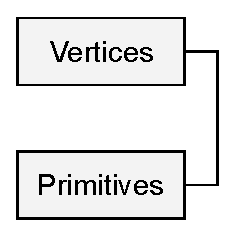
\includegraphics{images/ShaderTest.eps}
		\caption{Hello there shader test image}
		\label{fig:shadertest}
	\end{figure}
\end{section}

\begin{section}{Additional Section}
	Hello there some additional content of this section.
	
	\begin{equation}
		\begin{bmatrix}
			\cos{\theta} & -\sin{\theta} & 0 & 0 \\
			\sin{\theta} & \cos{\theta} & 0 & 0 \\
			0 & 0 & 1 & 0 \\
			0 & 0 & 0 & 1
		\end{bmatrix}
		\begin{bmatrix}
			x \\
			y \\
			z \\
			1
		\end{bmatrix}
	\end{equation}
\end{section}
	
\end{document}
